\chapter{Desenvolvimento}
\label{cap4}


Para dar inicio a esta fase, e com o objetivo de responder com eficacia aos requisitos identificados. Adotei neste ponto a metodologia de desenvolvimento agil \textit{Scrum}. Esta opção foi a que se adequou as necessidades de desenvolvimento deste projeto, pois ficou delineado que existiria uma reunião através do Microsoft Teams semanalmente, com o objetivo de compreender quais os progressos do sistema. 

Os papéis foram distribuídos da seguinte forma:
 
\begin{itemize}
  \item \textit{Product Owner}: o cliente;
  \item \textit{Scrum Master}: a professora Isabel Brito;
  \item \textit{Scrum Team} (equipa de desenvolvimento): Diogo Gonçalves.
\end{itemize}

A existência destes papéis foi fundamental, pois permitiu perceber, a cada reunião, o que deveria ser alterado em função das necessidades do cliente. Em cada reunião procurei ser claro na apresentação do ponto de situação, o que considero ter contribuído para o bom funcionamento do projeto.


\section{Processo ETL}
\label{sec:etl}

O ponto de partida do sistema é um ficheiro CSV (ou Excel) por sensor, do qual é necessário extrair os dados. A definição do que entra no sistema condiciona tudo o que é feito depois, pelo que esta foi uma das fases mais críticas do projeto. Para evitar redundância e garantir dados tão claros quanto possível, optou-se por um processo ETL (\textit{Extract, Transform and Load}) implementado em Python, com armazenamento em SQLite, exposto à aplicação Vue através de uma API REST em Flask.
 
\subsection{Extract}
\label{sec:etl-extract}

Na fase de extração, o ficheiro carregado é descodificado em UTF-8 (com ou sem \textit{BOM}), o separador (vírgula ou ponto e vírgula) é detetado automaticamente e as linhas são lidas como registos. É ainda verificado que os campos \texttt{timestamp\_init\_UTC} e \texttt{timestamp\_end\_UTC} existem, por serem indispensáveis; os restantes campos temporais podem ser reconstruídos.

\subsection{Transform}
\label{sec:etl-transform}


A transformação é feita linha a linha e inclui os seguintes passos:
 
\begin{itemize}
  \item \textbf{Normalização dos cabeçalhos}: as unidades são removidas do nome da coluna (por exemplo, \texttt{NO2(µg/m³)} passa a \texttt{NO2}), evitando também confundir \texttt{PM1} com \texttt{PM10};
  \item \textbf{Conversão de tipos}: os valores numéricos são convertidos para \textit{float} (aceitando vírgula decimal) e as datas para o formato ISO 8601 com fuso horário;
  \item \textbf{Coerência temporal}: o intervalo UTC tem de ter fim posterior ao início; as datas de Lisboa são recalculadas a partir das datas UTC com o fuso \texttt{Europe/Lisbon}, de modo a aplicar corretamente o horário de verão, e uma linha é rejeitada se o valor informado for incoerente com o UTC;
  \item \textbf{Validação de intervalos}: latitude entre $-90$ e $90$, longitude entre $-180$ e $180$, humidade entre 0 e 100\,\%, e ausência de valores negativos em poluentes e vento;
  \item \textbf{Valores em falta}: medições vazias são guardadas como \texttt{NULL}, nunca como zero, para não distorcer médias nem gráficos;
  \item \textbf{Deduplicação}: intervalos repetidos no mesmo ficheiro são rejeitados.
\end{itemize}
 
As linhas inválidas não interrompem a importação: ficam registadas num resumo de linhas rejeitadas, com o número da linha e o motivo.
 
A coluna \texttt{pressure} é indicada no CSV com a unidade \si{\micro\gram\per\cubic\metre}, o que é incoerente com valores como 984,5, que corresponderiam tipicamente a hPa. O ETL não converte nem assume unidades: o valor é armazenado tal como foi recebido, devendo a unidade ser confirmada junto da fonte dos dados.
 
 \subsection{Load}
\label{sec:etl-load}
 
Na fase de carga, cada ficheiro é inserido numa única transação SQLite: é criado ou consultado o sensor, é registado o ficheiro (o que impede importar duas vezes o mesmo ficheiro) e são inseridas as leituras. Qualquer erro de unicidade ou de SQL reverte a importação desse ficheiro, garantindo que não ficam dados parciais.
 
O modelo relacional 
\begin{figure}[htbp]
    \centering
    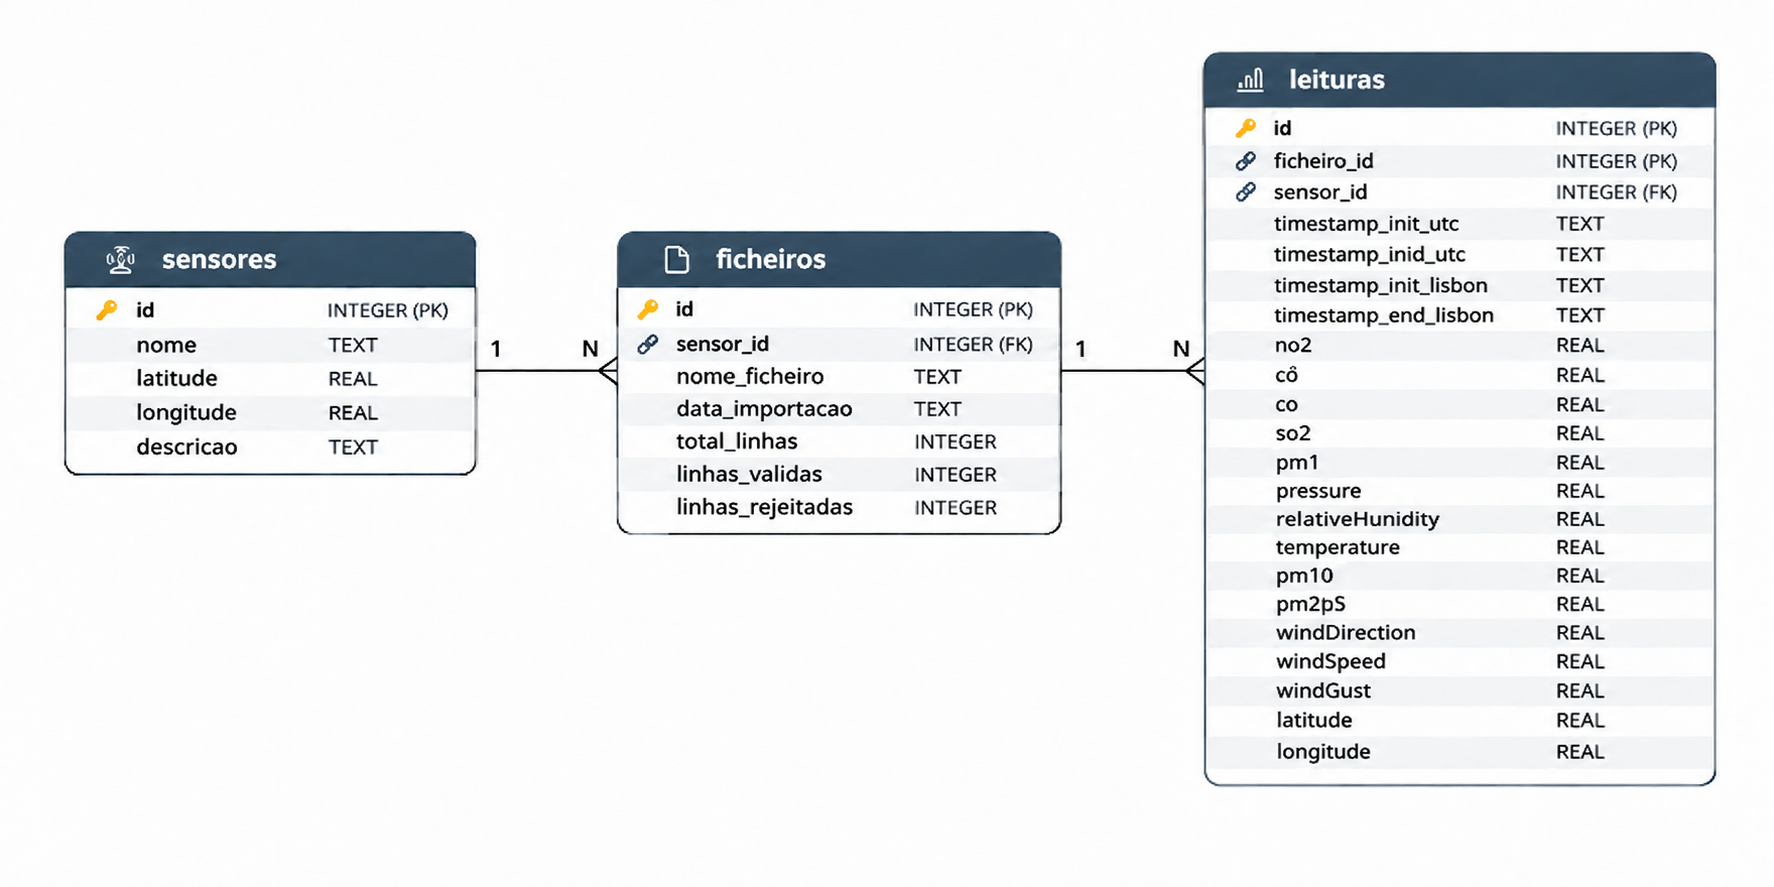
\includegraphics[width=\textwidth]{figuras/DiagramaBaseDeDados.png}
    \label{fig:modelo}
\end{figure} 
é composto por três tabelas:
 
\begin{itemize}
  \item \texttt{sensores}: identificador inteiro gerado automaticamente, nome, coordenadas, fuso horário, data de instalação e estado;
  \item \texttt{ficheiros}: nome do ficheiro importado, sensor associado e data de importação;
  \item \texttt{leituras}: uma linha por intervalo de medição, com chave estrangeira para o sensor e para o ficheiro, as quatro marcas temporais e os 15 campos numéricos (13 medições mais latitude e longitude).
\end{itemize}
 
A relação entre sensor e leituras é de um para muitos, e a restrição \texttt{UNIQUE(sensor\_id, timestamp\_init\_UTC, timestamp\_end\_UTC)} impede leituras duplicadas, enquanto um índice sobre sensor e tempo acelera as consultas mais frequentes.
 
% \begin{figure}[htbp]
%   \centering
%   \includegraphics[width=0.8\textwidth]{figuras/modelo_er}
%   \caption{Modelo relacional: sensores (1) $\rightarrow$ (N) leituras.}
%   \label{fig:modelo}
% \end{figure}
 
\subsection{Verificação}
\label{sec:etl-testes}
 
O processo ETL foi acompanhado por testes automáticos (\texttt{unittest}) que validam a leitura de uma linha de exemplo (valores numéricos e marcas temporais) e a rejeição de intervalos duplicados.
 
 
